\documentclass[a4paper,UTF8]{article}
\usepackage{ctex}
\usepackage[margin=1.25in]{geometry}
\usepackage{color}
\usepackage{graphicx}
\usepackage{amssymb}
\usepackage{amsmath}
\usepackage{amsthm}
\usepackage{tcolorbox}
\usepackage{enumerate}
\usepackage{hyperref}
\usepackage{subfigure}
%\usepackage[thmmarks, amsmath, thref]{ntheorem}
\theoremstyle{definition}
\newtheorem*{solution}{Solution}
\newtheorem*{prove}{Proof}
\usepackage{multirow}              

\setlength{\evensidemargin}{.25in}
\setlength{\textwidth}{6in}
\setlength{\topmargin}{-0.5in}
\setlength{\topmargin}{-0.5in}
% \setlength{\textheight}{9.5in}
%%%%%%%%%%%%%%%%%%此处用于设置页眉页脚%%%%%%%%%%%%%%%%%%
\usepackage{fancyhdr}                                
\usepackage{lastpage}                                           
\usepackage{layout}                                             
\footskip = 10pt 
\pagestyle{fancy}                    % 设置页眉                 
\lhead{2020年春季}                    
\chead{机器学习导论}                                                
% \rhead{第\thepage/\pageref{LastPage}页} 
\rhead{作业一}                                                                                               
\cfoot{\thepage}                                                
\renewcommand{\headrulewidth}{1pt}  			%页眉线宽,设为0可以去页眉线
\setlength{\skip\footins}{0.5cm}    			%脚注与正文的距离           
\renewcommand{\footrulewidth}{0pt}  			%页脚线宽,设为0可以去页脚线

\makeatletter 									%设置双线页眉                                        
\def\headrule{{\if@fancyplain\let\headrulewidth\plainheadrulewidth\fi%
		\hrule\@height 1.0pt \@width\headwidth\vskip1pt	%上面线为1pt粗  
		\hrule\@height 0.5pt\@width\headwidth  			%下面0.5pt粗            
		\vskip-2\headrulewidth\vskip-1pt}      			%两条线的距离1pt        
	\vspace{6mm}}     								%双线与下面正文之间的垂直间距              
\makeatother  

%--

%--
\begin{document}
\title{机器学习导论\\习题一}
\author{171830635, 俞星凯, yuxk@smail.nju.edu.cn}
\maketitle


\section*{学术诚信}

本课程非常重视学术诚信规范,助教老师和助教同学将不遗余力地维护作业中的学术诚信规范的建立。希望所有选课学生能够对此予以重视。\footnote{参考尹一通老师\href{http://tcs.nju.edu.cn/wiki/}{高级算法课程}中对学术诚信的说明。}

\begin{tcolorbox}
	\begin{enumerate}
		\item[(1)] 允许同学之间的相互讨论,但是{\color{red}\textbf{署你名字的工作必须由你完成}},不允许直接照搬任何已有的材料,必须独立完成作业的书写过程;
		\item[(2)] 在完成作业过程中,对他人工作(出版物、互联网资料)中文本的直接照搬(包括原文的直接复制粘贴及语句的简单修改等)都将视为剽窃,剽窃者成绩将被取消。{\color{red}\textbf{对于完成作业中有关键作用的公开资料,应予以明显引用}};
		\item[(3)] 如果发现作业之间高度相似将被判定为互相抄袭行为,{\color{red}\textbf{抄袭和被抄袭双方的成绩都将被取消}}。因此请主动防止自己的作业被他人抄袭。
	\end{enumerate}
\end{tcolorbox}

\section*{作业提交注意事项}
\begin{tcolorbox}
	\begin{enumerate}
		\item[(1)] 请在LaTeX模板中第一页填写个人的姓名、学号、邮箱信息;
		\item[(2)] 本次作业需提交该pdf文件、问题2问题4可直接运行的源码(两个.py文件)、作业2用到的数据文件 (为了保证问题2代码可以运行),将以上四个文件压缩成zip文件后上传,例如181221001.zip;
		\item[(3)] 未按照要求提交作业,或提交作业格式不正确,将会被扣除部分作业分数;
		\item[(4)] 本次作业提交截止时间为3月15日23:59:59。除非有特殊情况(如因病缓交),否则截止时间后不接收作业,本次作业记零分。
	\end{enumerate}
\end{tcolorbox}

\newpage
\section*{Problem 1}
若数据包含噪声,则假设空间中有可能不存在与所有训练样本都一致的假设,此时的版本空间是什么?在此情形下,试设计一种归纳偏好用于假设选择。
\begin{solution}
此处用于写解答(中英文均可)
~\\
~\\
从数据中选取最大子集,使得存在与其一致的假设,并且遵循归纳偏好选择假设:
\begin{itemize}
\item 如果存在多个基数相同的最大子集,那么选择与最早发现的最大子集一致的假设。
\item 如果存在多个与同一最大子集一致的假设,那么根据“奥卡姆剃刀”选择更“简单”的假设。
\item 如果存在多个同样“简单”的假设,那么任意选择一个假设。
\end{itemize}
\end{solution}

\section*{Problem 2 [编程]} 
现有500个测试样例,其对应的真实标记和学习器的输出值如表\ref{table:roc}所示 (完整数据见data.csv文件)。该任务是一个二分类任务,1表示正例,0表示负例。学习器的输出越接近1表明学习器认为该样例越可能是正例,越接近0表明学习器认为该样例越可能是负例。
\begin{table}[!h]
	\centering
	\caption{测试样例表} \vspace{2mm}\label{table:roc}
	\begin{tabular}{c|c c c c c c c c c c c}\hline
		样本 & $x_1$ & $x_2$ & $x_3$  & $x_4$  & $x_5$&...& $x_{496}$& $x_{497}$ & $x_{498}$ & $x_{499}$ & $x_{500}$ \\
		\hline
		标记 & 1  & 1 &  0 &  0  & 0 &... &0& 1 & 0 & 1 & 1\\
		\hline
		输出值 & 0.206  & 0.662 &  0.219 &  0.126  & 0.450 & ... & 0.184&0.505 & 0.445 & 0.994 & 0.602\\
		\hline
	\end{tabular}
\end{table}
\begin{enumerate}[ {(}1{)}]
\item 请编程绘制P-R曲线
\item 请编程绘制ROC曲线,并计算AUC
\end{enumerate}
本题需结合关键代码说明思路,并贴上最终绘制的曲线。建议使用Python语言编程实现。(预计代码行数小于100行)

提示:
\begin{itemize}
	\item 需要注意数据中存在输出值相同的样例。
	\item 
	在Python中,数值计算通常使用Numpy, 表格数据操作通常使用Pandas, 画图可以使用Matplotlib (Seaborn), 同学们可以通过上网查找相关资料学习使用这些工具。未来同学们会接触到更多的Python扩展库,如集成了众多机器学习方法的Sklearn, 深度学习工具包Tensorflow, Pytorch等。
\end{itemize}
\begin{solution}
此处用于写解答(中英文均可)	
\begin{verbatim}
data = data.sort_values('output', ascending=False)
thresholds = data['output'].unique()
n = len(thresholds)
for i in range(n):
    data['pred'] = data['output'] >= thresholds[i]
    TP = np.sum((data['label'] == 1) & (data['pred'] == 1))
    FP = np.sum((data['label'] == 0) & (data['pred'] == 1))
    TN = np.sum((data['label'] == 0) & (data['pred'] == 0))
    FN = np.sum((data['label'] == 1) & (data['pred'] == 0))
    P[i] = TP / (TP + FP)
    R[i] = TP / (TP + FN)
    TPR[i] = TP / (TP + FN)
    FPR[i] = FP / (FP + TN)
\end{verbatim}
先将数据按照\verb|output|从大到小排序,再依次取\verb|output|集合中的元素作为阈值,分别计算真正例、假正例、真反例、假反例,从而计算查准率、查全率、真正例率、假正例率。
\begin{verbatim}
AUC = np.sum((FPR[1:] - FPR[:-1]) * (TPR[:-1] + TPR[1:])) / 2
\end{verbatim}
AUC根据上面代码计算得到0.8737。
\begin{figure}[h]
	\centering
	\subfigure[P-R曲线]{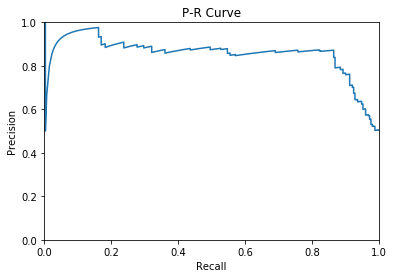
\includegraphics[scale=0.5]{P-R.png}}
	\subfigure[ROC曲线]{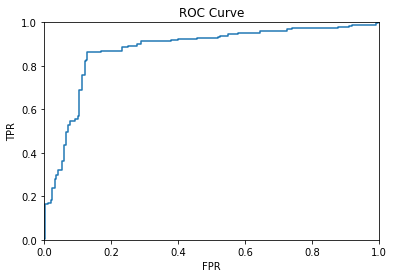
\includegraphics[scale=0.5]{ROC.png}}
	\caption{代码绘图}
\end{figure}
\end{solution}

\section*{Problem 3}
对于有限样例,请证明
\[
\text{AUC} = \frac{1}{m^+m^-}\sum_{x^+\in D^+}\sum_{x^-\in D^-}\left(\mathbb{I}(f(x^+)>f(x^-))+\frac{1}{2}\mathbb{I}(f(x^+)=f(x^-))\right)
\]

\begin{prove}
此处用于写证明(中英文均可)
~\\
~\\
将$m^+$个正例和$m^-$个反例分别按照预测值从大到小进行排序,分别记为$x_1^+,x_2^+,\cdots,x_{m^+}^+$\\和$x_1^-,x_2^-,\cdots,x_{m^-}^-$。考虑一个网格平面,纵坐标范围$[0,m^+]$,横坐标范围$[0,m^-]$。对于任意$1\times1$网格,根据其右上角顶点$(i,j)$,按照如下规则染色:
\begin{itemize}
\item $f(x_j^+)>f(x_i^-)$,将整个网格染色。
\item $f(x_j^+)<f(x_i^-)$,不染色。
\item $f(x_j^+)=f(x_i^-)$,将网格左下、右上、右下三点组成的三角形染色。
\end{itemize}
因为小正方形面积为$1$,小三角形面积为$\frac12$,所以染色区域面积为:
\[\sum_{x^+\in D^+}\sum_{x^-\in D^-}\left(\mathbb{I}(f(x^+)>f(x^-))+\frac{1}{2}\mathbb{I}(f(x^+)=f(x^-))\right)\]
修正染色区域,若$a$个正例和$b$个反例预测值相同,即存在宽为$a$,长为$b$的矩形,其中所有网格都是三角形染色,则对该矩形重新染色,将矩形左下、右上、右下三点组成的三角形染色。注意修正前后,该矩形染色面积都为$\frac12ab$,因此修正之后的染色区域面积不变。
\begin{figure}[h]
	\centering
	\subfigure[染色图示]{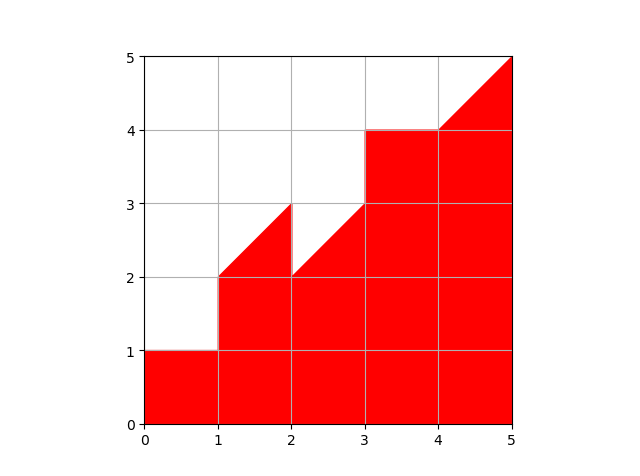
\includegraphics[scale=0.45]{Grid.png}}
	\subfigure[修正图示]{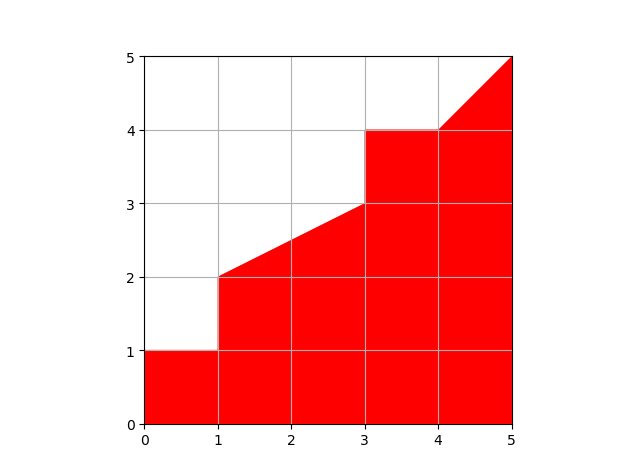
\includegraphics[scale=0.45]{Grid2.png}}
	\caption{染色与修正,样例满足$x_1^+>x_1^->x_2^+>x_2^-=x_3^+=x_3^->x_4^+>x_4^->x_5^+=x_5^-$}
\end{figure}\\
将坐标系的横纵坐标范围都缩小到$[0,1]$,这时染色区域面积缩小$m^+m^-$倍。考虑染色区域左边界上的点$(x,y)$,对应原来网格平面上的点$(i,j)$。若将满足$f(x)\geq max\{f(x_i^-),f(x_j^+)\}$的样例预测为正例,其余预测为反例,则$x$是假正例率,$y$是真正例率,于是所有这些点构成ROC曲线。又根据小于关系传递性,染色区域内部不存在空白,故AUC即为染色区域面积:
\[
\text{AUC} = \frac{1}{m^+m^-}\sum_{x^+\in D^+}\sum_{x^-\in D^-}\left(\mathbb{I}(f(x^+)>f(x^-))+\frac{1}{2}\mathbb{I}(f(x^+)=f(x^-))\right)
\]
\qed
\end{prove}

\section*{Problem 4 [编程]} 
在数据集$D_1,D_2,D_3,D_4,D_5$运行了$A,B,C,D,E$五种算法,算法比较序值表如表\ref{table:ranking}所示:
\begin{table}[h]
\centering
\caption{算法比较序值表} \vspace{2mm}\label{table:ranking}
\begin{tabular}{c|c c c c c}\hline
数据集 & 算法$A$ & 算法$B$  & 算法$C$  &算法$D$  &算法$E$ \\
\hline
$D_1$ & 2  & 3 &  1 &  5  & 4\\
$D_2$ & 5  & 4 &  2 &  3  & 1\\
$D_3$ & 4  & 5 &  1 &  2  & 3\\
$D_4$ & 2  & 3 &  1 &  5  & 4\\
$D_5$ & 3  & 4 &  1 &  5  & 2\\
\hline
平均序值 & 3.2 &  3.8 & 1.2 &  4 &  2.8 \\
\hline
\end{tabular}
\end{table}

使用Friedman检验$(\alpha=0.05)$判断这些算法是否性能都相同。若不相同,进行Nemenyi后续检验$(\alpha=0.05)$,并说明性能最好的算法与哪些算法有显著差别。本题需编程实现Friedman检验和Nemenyi后续检验。(预计代码行数小于50行)
\begin{solution}
此处用于写解答(中英文均可)
\begin{verbatim}
# Friedman检验
r = data.mean()
n, k = data.shape
chi2 = 12 * n / k / (k + 1) * (np.sum(r ** 2) - (k * (k + 1) ** 2) / 4)
fvalue = (n - 1) * chi2 / (n * (k - 1) - chi2)
if fvalue < f.ppf(0.95, 4, 16):
    print("所有算法性能相同")
# Nemenyi检验
else:
    cd = 2.728 * np.sqrt(k * (k + 1) / 6 / n)
    for i in range(k):
        for j in range(i + 1, k):
            if abs(r[i] - r[j]) > cd:
                print(f'算法{r.index[i]}与{r.index[j]}性能显著不同')
\end{verbatim}
代码根据西瓜书公式实现,性能最好的是算法$C$,与算法$D$有显著区别。
\end{solution}
\end{document}